\chapter{Energiemessung}

Zuerst f�hren wir eine Energiemessung des
Elektronenstrahls mithilfe
eines Dipolmagneten durch. Die
Elektronen, aus dem der Strahl besteht, werden
am Anfang des Beschleunigers thermisch durch die Kathode erzeugt
und erhalten so ihre kinetische Energie und ihren Impulsbetrag,
die sie von da an behalten, da sie im Beschleuniger nur mit den
Feldern der Dipol- und Quadrupolmagnete �ber die Lorentzkraft
wechselwirken.

Die Energiemessung geschieht, indem der Zusammenhang zwischen
Ablenkung durch einen der Dipole und St�rke des Dipols gemessen
wird, da erstere theoretisch linear von der letzteren abh�ngt.
Genauer gilt:

Sei $L_{eff}$ die L�nge des Einflussbereichs des Dipols, sei dahinter
eine Driftstrecke mit L�nge $L_{drift}$ und am Ende ein Schirm. Sei
$x$ der Versatz des Strahls auf dem Schirm in die Richtung,
in die er vom Dipol abgelenkt wird. Es gilt dann
$x = x_0 + \frac{dx}{dI} I$, wobei $x_0$ der Versatz auf dem Schirm
ohne Wirkung des Dipols ist. (Man bedenke, dass $\frac{dx}{dI}$ negativ
sein kann.) $I$ ist der
Strom des Dipols und dieser ist proportional zur Dipolfeldst�rke $B$.
Es gibt also ein $\kappa$ so, dass $\kappa I = B L_{eff}$.
Sei $v$ die Geschwindigkeit der auf den
Schirm treffenden Elektronen, $\beta := \frac{v}{c}$, $c$ die Lichtgeschwindigkeit,
$\gamma := \frac{1}{\sqrt{1-\beta^2}}$, $m_e$ die Elektronenmasse und $e$
die Elementarladung.
Dann gilt:

\begin{equation} \label{eq:dipolabl}
	\beta \gamma = \frac{e \kappa L_{drift} }
	                    {m_e c |\frac{dx}{dI}|}
\end{equation}

Wir messen eine Reihe von Wertepaaren f�r $I$ und $x$, indem wir zuerst mit Blick
auf das Kamerabild des Schirms 3 ein Intervall f�r den Dipolstrom $I$ aussuchen,
bei dem der Strahl ganz auf dem Schirm zu sehen ist. Dann messen wir f�r
$(0,05\text{ A})$-Schritte innerhalb dieses Intervalls Werte f�r $x$
mit den Messergebnissen,
die in Tabelle \ref{tab:dipolabl} dargestellt sind. Die Messung wird dabei so
durchgef�hrt, dass zuerst der Strahl ganz vom Schirm abgelenkt wird, indem der Strom
des horizontalen Dipols V14NJ um 1 A verstellt wird. Dann wird von der Kamera ein
Bild aufgenommen (durch Mittelung �ber 50 frames), welches im Folgenden als
Hintergrund von den Bildern mit Strahl abgezogen wird. Das Bildanalyse-Programm
ermittelt
dann jeweils nach Mittelung �ber 20 frames die $x$-Position des Intensit�tsmaximums,
welches der Strahlmitte entspricht, nachdem mit der Maus ein enger Bereich um
den Strahlfleck im Kamerabild abgegrenzt wird.

Aus den Messwerten in Tabelle \ref{tab:dipolabl} ermitteln wir mithilfe
linearer Regression einen Wert f�r $\frac{dx}{dI}$,
woraus wir mit \eqref{eq:dipolabl} einen Wert f�r $\beta \gamma$ erhalten.
Wir finden $\frac{dx}{dI} = -0,0147 \pm 0,0002 \frac{\text{m}}{\text{A}}$ 
(siehe hierzu auch Abbildung \ref{linreg}) und
daraus mit Fehlerfortpflanzung $\beta\gamma = 0,168 \pm 0,002$.
Wegen $\gamma = \sqrt{1+\beta^2\gamma^2}$
erhalten wir damit $\gamma = 1,0139 \pm 0,0004$.

\begin{table}[ht]
\centering
\begin{tabular}{| >{$}c<{$} >{$}c<{$} |}
\hline
I\text{ [A]}	&		x\text{ [mm]}	 \\ [0.2ex]
\hline\hline
-3,50	&		4,07	 \\
-3,45	&		3,41	 \\
-3,40	&		2,71	 \\
-3,35	&		2,05	 \\
-3,30	&		1,23	 \\
-3,25	&		0,37	 \\
-3,20	&		-0,10	 \\
-3,15	&		-0,58	 \\
-3,10	&		-1,44	 \\
-3,05	&		-2,19	 \\
-3,00	&		-2,85	 \\
-2,95	&		-3,55	 \\
-2,90	&		-4,16	 \\
-2,85	&		-5,05	 \\
-2,80	&		-6,21	 \\
-2,75	&		-6,82	 \\
-2,70	&		-7,85	 \\
-2,65	&		-8,56	 \\
-2,60	&		-9,21	 \\
-2,55	&		-9,78	 \\
-2,50	&		-10,17	 \\
\hline
\end{tabular}
\caption{Messung des horizontalen Versatzes $x$ auf Schirm 3 bei Ablenkung
		durch den Dipol H15Match betrieben mit Strom $I$.}
	\label{tab:dipolabl}
\end{table}

\begin{figure}[ht]
    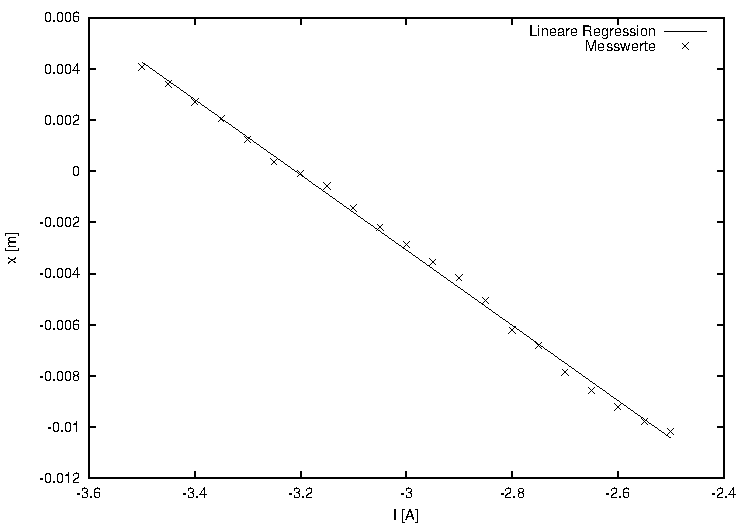
\includegraphics[width=1\textwidth]{./energiemessung.pdf}
	\caption{Messwerte aus Tabelle \ref{tab:dipolabl} mit Regressionsgerade
	gegeben durch $x = -0,0147 \cdot I - 0,0472$.} \label{linreg}
\end{figure}

Da $\gamma = \frac{E}{m_e c^2} = 1 + \frac{E_{\text{kin}}}{m_e c^2}$ gilt,
wenn $E$ die Gesamtenergie des einzelnen Elektrons ist, erhalten wir
schliesslich f�r seine kinetische Energie $E_{\text{kin}} = 7,1 \pm 0,2
\text{ keV}$,
wobei wir den Literaturwert $m_e c^2 = 511\text{ keV}$ verwenden. Wir erhalten
dann f�r den Impuls
$p = m_e c^2 \gamma \beta \frac{1}{c} = 85,6 \pm 1,2 
\frac{1}{\text{c}} \text{keV}$.

